\documentclass[10pt]{beamer}

\usepackage{minted}
\usepackage{booktabs}
\usepackage{tikz}
\usetikzlibrary{arrows.meta,decorations.markings}
\usetheme{default}

\AtBeginSection[]{
	\begin{frame}
		\vfill
		\centering
		\begin{beamercolorbox}[sep=8pt,center,shadow=true,rounded=true]{title}
			\usebeamerfont{title}\insertsectionhead\par%
		\end{beamercolorbox}
		\vfill
	\end{frame}
}

\title{Programming in parallel}
\subtitle{A (quick) overview}
\author{Pierre Beaujean (Belgian NCC for HPC)}
\date{v0.1a, November 2021}

\newminted{c}{tabsize=2,bgcolor=gray!10,fontsize=\small}
\newminted{text}{tabsize=2,bgcolor=gray!10,fontsize=\small}

\begin{document}
	
	\maketitle

\newcommand{\cdx}[1]{\textcolor{blue!75!black!85}{\texttt{\itshape #1}}}
	
\begin{frame}{About me}
	\framesubtitle{
		\url{https://pierrebeaujean.net/}}
	\begin{itemize}
		\item 2006: Ubuntu 6.06 LTS, from a friend
		\item 2007: Started learning programming from the \textit{Site du Zéro} (now deceased!).
		\item 2009: chose to study chemistry instead, but keeps Linux
		\item 2015: Switching to \textit{Zeste de Savoir} (I'm still there!)
		\item January 2015: Started and fulfilled a master’s thesis in Quantum Chemistry
		\item September 2015: started (and recently fulfilled!) a PhD in Quantum Chemistry, as Teaching Assistant
		\item September 2017: started (and fulfilled) a bachelor in computer science (evening classes)
		\item September 2021: started to work for the Belgian NCC for HPC.
	\end{itemize}
	
\end{frame}

\begin{frame}{Preliminary notes}
	\begin{itemize}
		\item Jokes and opinions are my own, not the one of the NCC Belgium ;)
		\item First of all, ``Premature optimization is the root of all evil'' (Sir Tony Hoare)
		\item Code optimization is an art, and the result depends on the target architecture (cache size, instruction set, connectivity, etc. See \cdx{lscpu}).
		\item Here, we will not look for the best optimized code (i.e., using manual optimization techniques such as manual loop unrolling or writing asm). We will just look at the effect of some modifications (and sometimes, the assembler).
		\item Codes are in C (but could be in Fortran), compiled with \cdx{gcc} (Intel compiler may provide better results on Intel architectures). 
		\item Two simple examples from linear algebra (LAPACK): \cdx{*dot} and \cdx{*axpy}. If you ever need that, use libraries instead!
	\end{itemize}
\end{frame}

\begin{frame}[fragile]{The examples for today}
	\begin{itemize}
		\item \cdx{(s|d)dot}: dot product of two vectors: $r = \vec{x}\cdot\vec{y}$.
		\begin{ccode}
float sdot(int n, float* x, float* y) {
	float sum = .0f;
	if (n > 0) {
		for(int i=0; i < n; i++)
			sum += y[i] * x[i];
	}
	return accum;
}
		\end{ccode}
	Note: actually use a \textbf{Kahan sum}!
		\item \cdx{(s|d)axpy}: generalized vector addition: $\vec y = \vec y + a\,\vec x$.
		\begin{ccode}
void saxpy(int n, float alpha, float* x, float* y) {
	if (n > 0 && alpha != 0.f) {
		for(int i=0; i < n; i++)
			y[i] += alpha * x[i];
	}
}
		\end{ccode}
	\end{itemize}
\end{frame}

\begin{frame}[fragile]{Preamble: Kahan sum}
	\url{https://en.wikipedia.org/wiki/Kahan_summation_algorithm}
	\begin{columns}
	\column[t]{.65\textwidth}
	\begin{ccode}
float sdot(int n, float* x, float* y) {
	float sum = .0f, c = .0f;
	float addend, tmpSum;
	if (n > 0) {
		for(int i=0; i < n; i++) {
			addend = y[i] * x[i] - c;
			tmpSum = sum + addend;
			c = (tmpSum - sum) - addend;
			sum = tmpSum;
		}
	}
	return sum;
}
	\end{ccode}
\column[t]{.35\textwidth}
	\begin{center}
		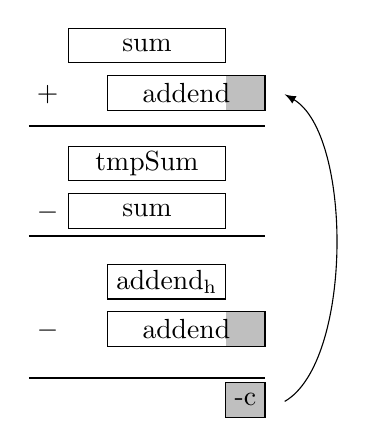
\begin{tikzpicture}
			\draw (0,0) rectangle +(2,1.25em) node[midway]{\cdx{sum}};
			\fill[black!25] (2,-.6) rectangle +(.5,1.25em);
			\draw (.5,-.6) rectangle +(2,1.25em) node[midway]{\cdx{addend}};
			\draw (0,-.4)  node[left]{$+$};
			\draw[thick] (-.5,-.8) -- +(3,0);
			\draw (0,-1.5) rectangle +(2,1.25em) node[midway]{\cdx{tmpSum}};
			\draw (0,-2.1) rectangle +(2,1.25em) node[midway]{\cdx{sum}};
			\draw (0,-1.9)  node[left]{$-$};
			\draw[thick] (-.5,-2.2) -- +(3,0);
			\draw (.5,-3) rectangle +(1.5,1.25em) node[midway]{\cdx{addend}\textsubscript{h}};
			\fill[black!25] (2,-3.6) rectangle +(.5,1.25em);
			\draw (.5,-3.6) rectangle +(2,1.25em) node[midway]{\cdx{addend}};
			\draw (0,-3.4)  node[left]{$-$};
			\draw[thick] (-.5,-4) -- +(3,0);
			\draw[fill=black!25] (2,-4.5) rectangle +(.5,1.25em) node[midway]{-\cdx{c}};
			\draw[-latex] (2.75,-4.3) .. controls +(30:1) and +(-30:1) .. (2.75,-.4);
		\end{tikzpicture}
	\end{center}
\end{columns}
\end{frame}

\begin{frame}{Preamble: don't forget 'bout optimization}
	\begin{table}
		\begin{tabular}{l cc c cc}
			\toprule
			& \multicolumn{2}{c}{\cdx{*dot}} &&\multicolumn{2}{c}{\cdx{*axpy}}\\
			& \cdx{s} & \cdx{d} && \cdx{s} & \cdx{d}\\
			\midrule
			\cdx{-O0} & 426.5 & 420.4 && 137.3 & 136.4\\
			\cdx{-O1} & 141.1 & 140.1  && 30.7 & 31.7\\
			\bottomrule
		\end{tabular}
		\caption{Average running times (in ms) with \cdx{-N 1000}, on $2^{24}$ numbers.}
	\end{table}
	\begin{itemize}
		\item Ran on AMD EPYC 7542, and compiled with GCC 10.2
		\item Compilers does a decent job at optimizing (see \url{https://gcc.gnu.org/onlinedocs/gcc/Optimize-Options.html} for the details)
		\item \cdx{-O2} and \cdx{-O3} include stuff we will see later on (but you \textbf{should} use \cdx{-O3}, or even \cdx{-Ofast}).
		\item If you are brave enough \cdx{objdump -dS -M intel <program, compiled with -g>}. Here, gcc chooses to use \cdx{muls(s|d)} (from the old SSE extension).
	\end{itemize}
\end{frame}
\section{``SIMD for nothin', FLOPS for free'' (old song)}

\begin{frame}{SIMD}
	\begin{itemize}
		\item SIMD = ``simple instruction, multiple data'' (in Flynn's taxonomy). Correspond to data level parallelism.
		\item Refers to (at least) two mechanisms: pipelining\footnote{See ``Fonctions et concepts des ordinateurs'' (INFOB2126/IHDCB142)} and \textbf{packed instruction} / vector processing.
		\item Response to early graphic cards: MMX (64 bits registers, for integers) / 3DNow! (+\cdx{float}) \textrightarrow{} SSE (128 bit registers, +\cdx{double}) \textrightarrow{} AVX (256 and 512 bit registers)
		\item Example: SSE\begin{center}
			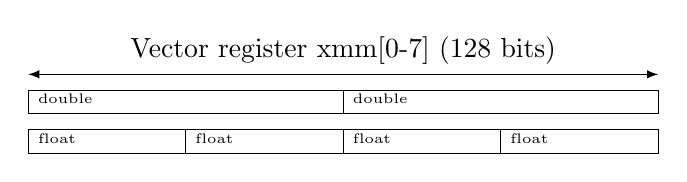
\begin{tikzpicture}
				\draw[latex-latex] (0,0) -- +(8,0) node[midway,above]{Vector register \cdx{xmm[0-7]} (128 bits)};
				\draw (0,-.5) node[anchor=south west]{\tiny \cdx{double}} rectangle +(4,.3);
				\draw (4,-.5) node[anchor=south west]{\tiny \cdx{double}} rectangle +(4,.3);
				\draw (0,-1) node[anchor=south west]{\tiny \cdx{float}} rectangle +(2,.3);
				\draw (2,-1) node[anchor=south west]{\tiny \cdx{float}} rectangle +(2,.3);
				\draw (4,-1) node[anchor=south west]{\tiny \cdx{float}} rectangle +(2,.3);
				\draw (6,-1) node[anchor=south west]{\tiny \cdx{float}} rectangle +(2,.3);
			\end{tikzpicture}
		\end{center}
	\end{itemize}
\end{frame}

\begin{frame}[fragile]{Vector processing}
	Examples with SSE (as modified by AVX):
	\begin{ccode}
float x[N], y[N], z[N];
for(i=0; i < N; i++)
	z[i] = x[i] + y[i];
	\end{ccode}
	The last line is translated into \texttt{vaddps} \textcolor{blue}{\texttt{xmm1}},\textcolor{red}{\texttt{xmm2}},\textcolor{green}{\texttt{xmm3}} (among other things).
	\begin{center}
		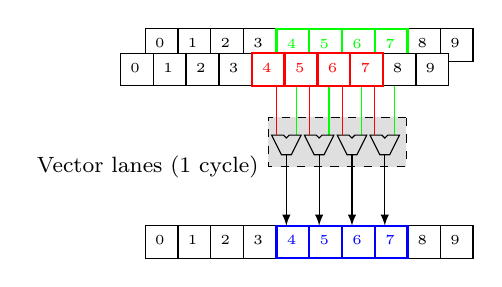
\begin{tikzpicture} [scale=1.25,rotate=-90]
			\draw[dashed,fill=gray!25] (.9,2.65)  rectangle +(.5,-1.4)node[left]{\footnotesize Vector lanes (1 cycle)};
			\foreach\i in {0,1,2,3,8,9} {
				\draw (0,\i / 3) node[anchor=north west]{\tiny \i} rectangle +(.33,.33);	
				\draw (2,\i / 3) node[anchor=north west]{\tiny \i} rectangle +(.33,.33);
			}
			\foreach\i in {4,5,6,7} {
				\draw[green,thick] (0,\i / 3) node[anchor=north west]{\tiny \i} rectangle +(.33,.33);	
				\draw[blue,thick] (2,\i / 3)  node[anchor=north west]{\tiny \i} rectangle +(.33,.33);
				\draw[green] (.33,\i / 3 + .2) -- ++(.75,0);
				\draw (1.08, \i / 3 + .25) -- ++(.2,-.1) -- ++(0,-.1) -- ++(-.2,-.1)  -- ++(0,.12)-- ++(.03,.03) -- ++(-.03,.03) -- cycle;
				\draw[-latex] (1.28,\i / 3 + .1) -- (2,\i / 3 + .1);
			}
			\foreach\i in {0,1,2,3,8,9} {
				\draw[fill=white] (.25,\i / 3 - .25) node[anchor=north west]{\tiny \i} rectangle +(.33,.33);
			}
			\foreach\i in {4,5,6,7} {	
				\draw[red,fill=white,thick] (.25,\i / 3 - .25) node[anchor=north west]{\tiny \i} rectangle +(.33,.33);
				\draw[red] (.58,\i / 3) -- ++(.5,0); 
			}
		\end{tikzpicture}
	\end{center}
	The program runtime for this part is (theoretically!) divided by the number of vector lanes.
\end{frame}

\begin{frame}[fragile]{Howto!}
	\begin{itemize}
		\item Write assembler (\textbf{don't!})
		\item Use compiler intrinsic (if you \textbf{really} have to):\begin{ccode}
#include <xmmintrin.h>
__m128 r1 = _mm_load_ps(&x[4*i]);
__m128 r2 = _mm_load_ps(&y[4*i]);
__m128 r0 = _mm_add_ps(r1, r2);
_mm_store_ps(&z[4*i],r0);
		\end{ccode}
		\item Use SIMD classes (in C++)
		\item Add \cdx{\#pragma omp simd} above the loop (other exists, but it depends on the compiler) and compile with \cdx{-fopenmp-simd} (gcc).
		\item Let the compiler do its job ... And maybe check its result. With gcc, \cdx{-ftree-vectorize} (or \cdx{-O2}) and \cdx{-fopt-info-loop-(optimized|missed)}. The compiler may refuse to optimize a loop, though.
	\end{itemize}
\end{frame}

\begin{frame}[fragile]{Aliasing?}
	
	\begin{itemize}
		\item If one compiles the serial code of the \cdx{axpy} example, the output is something like\begin{textcode}
1_serial.c:11:9: optimized: loop vectorized using 16 byte
vectors
1_serial.c:11:9: optimized:  loop versioned for 
vectorization because of possible aliasing
(...)
		\end{textcode}
		So the loop (here the one of \cdx{saxpy}) get vectorized (with 16-byte vector, so a 128 bit register), but also versioned.
		\item Here, the compiler is not able to determine whether \cdx{x} and \cdx{y} point to the same memory address, so it keeps both versions (and will choose at runtime).
		\item Use \cdx{restrict} to help:\begin{ccode}
void saxpy(int n, float alpha, 
	float* restrict x, float* restrict y) 
		\end{ccode}
	\end{itemize}
\end{frame}

\begin{frame}{Results}
	\begin{table}
		\begin{tabular}{p{4.5cm}lll}
			\toprule
			&Instruction& \cdx{saxpy} & \cdx{daxpy} \\
			\midrule
			\cdx{\small -O1} & \cdx{mulsd} & 30.7 & 31.7 \\
			\cdx{\small -O1 -ftree-vectorize} & \cdx{mulpd} & 16.0 & 27.3 \\
			\cdx{\small -O1 -lm -ftree-vectorize -mavx2} & \cdx{vmulpd} + 2 l.u. & 16.2 & 27.3 \\
			\cdx{\small -O1 -ftree-vectorize \mbox{-m}arch=native -mtune=native}  & \cdx{vmulpd} + 4 l.u. & 14.5 & 25.8 \\
			\bottomrule
		\end{tabular}
	\caption{Instruction for multiplication of double and average running times (in ms) with \cdx{-N 1000}, on $2^{24}$ numbers.}
	\end{table}
\begin{itemize}
	\item Use \cdx{-march=native -mtune=native} for best performances.
	\item \cdx{dot} does not vectorize ... \textbf{Why?}
\end{itemize}
\end{frame}
\section{Threading made easy: OpenMP}

\begin{frame}{Threads}
	\begin{itemize}
		\item Reminder: a thread is an independent sequence of instructions that can be managed by a scheduler. Multiple threads can exist for one process, with shared memory. May induce \textbf{race conditions} (e.g., data race).
		\item Using dedicated libraries (e.g., pthreads) may be cumbersome, especially since, in scientific computing, the paradigm is usually different.\begin{center}
			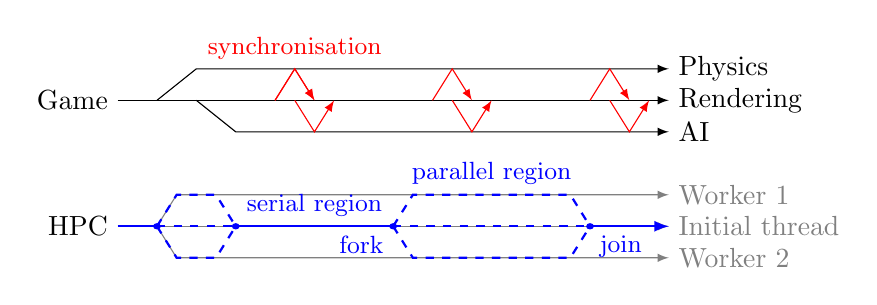
\begin{tikzpicture}[yscale=.8]
				\draw[-latex] (0,0) node[left]{Game} -- +(7,0) node[right]{Rendering};
				\draw[-latex] (.5, 0) -- ++(.5,.5) --  ++(6,0)node[right]{Physics};
				\draw[-latex] (1, 0) -- ++(.5,-.5) --  ++(5.5,0) node[right]{AI};
				\draw [red, -latex] (2,0) -- ++(.25,.5) -- ++(.25,-.5);
				\draw [red, -latex] (2,0) -- ++(.25,.5) node[above]{\small synchronisation} -- ++(.25,-.5);
				\draw [red, -latex] (2.25,0) -- ++(.25,-.5) -- ++(.25,.5);
				\draw [red, -latex] (4,0) -- ++(.25,.5) -- ++(.25,-.5);
				\draw [red, -latex] (4.25,0) -- ++(.25,-.5) -- ++(.25,.5);
				\draw [red, -latex] (6,0) -- ++(.25,.5) -- ++(.25,-.5);
				\draw [red, -latex] (6.25,0) -- ++(.25,-.5) -- ++(.25,.5);
				\begin{scope}[yshift=-2cm]
					\draw[-latex,gray] (0,0) node[left,black]{HPC} -- +(7,0) node[right]{Initial thread};
					\draw[-latex,gray] (.5, 0) -- ++(.25,.5) --  ++(6.25,0)node[right]{Worker 1};
					\draw[-latex,gray] (.5, 0) -- ++(.25,-.5) --  ++(6.25,0)node[right]{Worker 2};
					
					\draw[blue,thick] (0,0) -- ++(.5,0);
					\fill[blue] (.5,0) circle (.05cm);
					\draw[blue,dashed,thick] (.5,0) -- ++(.25,.5) -- ++(.5,0) -- ++(.25,-.5);
					\draw[blue,dashed,thick] (.5,0) -- ++(1,0);
					\draw[blue,dashed,thick] (.5,0) -- ++(.25,-.5) -- ++(.5,0) -- ++(.25,.5);
					\fill[blue] (1.5,0) circle (.05cm);
					\draw[blue,thick] (1.5,0) -- ++(2,0) node[midway,above]{\small serial region};
					\fill[blue] (3.5,0) circle (.05cm) node[anchor=north east]{\small fork};
					\draw[blue,dashed,thick] (3.5,0) -- ++(.25,.5) -- ++(2,0) node[midway,above]{\small parallel region} -- ++(.25,-.5);
					\draw[blue,dashed,thick] (3.5,0) -- ++(2.5,0);
					\draw[blue,dashed,thick] (3.5,0) -- ++(.25,-.5) -- ++(2,0) -- ++(.25,.5);
					\fill[blue] (6,0) circle (.05cm) node[anchor=north west]{\small join};
					\draw[blue,-latex,thick] (6,0) -- ++(1,0);
				\end{scope}
			\end{tikzpicture}
		\end{center}
		\item OpenMP is built on the fork/join paradigm, and generally does not use synchronization.
	\end{itemize}
\end{frame}

\begin{frame}[fragile]{OpenMP}
	\begin{itemize}
		\item Main paradigm in scientific computing for single-node applications!
		\item To use OpenMP, add directives (\cdx{\#pragma omp}) and rely on the compiler for the underlying details. One of the advantages is that it allows an \textbf{incremental} adoption.
		\item But, of course, there are still two problems that the compiler cannot solve on its own: \begin{enumerate}
			\item data dependencies:\begin{ccode}
for(i=2;i<N;i++) // Vietnam flashback, anyone?
	a[i] = a[i-1] + a[i-2];
			\end{ccode}
			\item data race (more on that later):\begin{ccode}
int x = 0;
for(i=0;i<N;i++)
	x = x + a[i];
			\end{ccode}
		\end{enumerate}
	\end{itemize}
\end{frame}

\begin{frame}[fragile]{Hello, world!}
	\begin{ccode}
#include <stdio.h>
#include <omp.h>

int main() {
	#pragma omp parallel
	{ // fork!
		printf("I'm thread %d of %d\n",
			omp_get_thread_num(), omp_get_num_threads());
	} // implicit join
}
	\end{ccode}
	Compile and execute:
	\begin{textcode}
$ gcc -o hello hello.c -fopenmp
$ OMP_NUM_THREADS=4 ./hello
I'm thread 0 of 4
I'm thread 2 of 4
I'm thread 3 of 4
I'm thread 1 of 4
	\end{textcode}
\end{frame}

\begin{frame}[fragile]{Parallel $\neq$ Worksharing }
	\begin{itemize}
		\item The content of the parallel region is executed by all threads:\begin{ccode}
#pragma omp parallel
{
	for(i=0;i<N;i++)
		a[i] = a[i]+ 1;
} // each thread execute the N iterations
		\end{ccode}
		\item Explicit work sharing:\begin{ccode}
#pragma omp parallel
{
	int t = omp_get_thread_num();
	int n = omp_get_num_threads();
	int low = N * t / n, high = N * (t + 1) / n;
	for(int i = low; i < high; i++)
		a[i] = a[i] + 1;
} // each thread do its part
		\end{ccode}
	\end{itemize}
\end{frame}

\begin{frame}[fragile]{Parallel $\neq$ Worksharing}
	But there is an easier way:
	\begin{itemize}
		\item With a directive...\begin{ccode}
#pragma omp parallel
{
	#pragma omp for
	for(i=0;i<N;i++)
		a[i] = a[i]+ 1;
} // each thread do its part
		\end{ccode}
		\item ... And directives can be combined:\begin{ccode}
#pragma omp parallel for
for(i=0;i<N;i++)
	a[i] = a[i]+ 1; // no curly braces required, but barrier
		\end{ccode}
	\end{itemize}
	Note: of course, \cdx{\#pragma omp for} must be in a parallel region (otherwise, it is only bound to the master thread). It may be useful for \textbf{orphaning}, though.
\end{frame}

\begin{frame}[fragile]{Say hello to data race!}
	\begin{ccode}
#include <stdio.h>
#include <omp.h>

int main() {
	int i, n; // ... why not?
	#pragma omp parallel
	{
		i = omp_get_thread_num(); n = omp_get_num_threads();
		printf("I'm thread %d of %d\n", i, n);
	}
}
	\end{ccode}
	Compile and execute gives (sometimes\footnote{Data race is difficult to spot, since they do not happen every time ;)}):
	\begin{textcode}
$ OMP_NUM_THREADS=4 ./hello
I'm thread 2 of 4
I'm thread 2 of 4
I'm thread 3 of 4
I'm thread 2 of 4
	\end{textcode}
\end{frame}

\begin{frame}[fragile]{First problem: communism. Let's privatize!}
	\begin{itemize}
		\item Any variable declared outside a parallel region is shared by default.
		\item Either we declare them inside:\begin{ccode}
#pragma omp parallel
{
	int i = omp_get_thread_num(); // private
	int n = omp_get_num_threads(); // private
	printf("I'm thread %d of %d\n", i, n);
}
		\end{ccode}
		\item Or we use the \cdx{private(list)} clause:\begin{ccode}
int i, n;
#pragma omp parallel private(i,n)
{
	i = omp_get_thread_num();
	n = omp_get_num_threads();
	printf("I'm thread %d of %d\n", i, n);
}
		\end{ccode}
	\end{itemize}
\end{frame}

\begin{frame}[fragile]{Privatization issue: initial value}
	\begin{ccode}
int i = 1;
#pragma omp parallel private(i)
printf("Value is %d\n", i + 1);
	\end{ccode}
	gives\begin{textcode}
$ OMP_NUM_THREADS=1 ./tmp
Value is 1
	\end{textcode}
	Why? Because private variables are \textbf{not} initialized by default in the parallel region. You should use \cdx{firstprivate}, which initialize to its value in the main thread, for that:\begin{ccode}
i = 1;
#pragma omp parallel firstprivate(i)
printf("Value is %d\n", i + 1);
	\end{ccode}
	which gives\begin{textcode}
$ OMP_NUM_THREADS=1 ./tmp
Value is 2
	\end{textcode}
\end{frame}

\begin{frame}[fragile]{Second problem: communism IS usefull!}
	\begin{ccode}
int sum = 0;
#pragma omp parallel for
for (int i=0; i < N; i++)
	sum += a[i]; // numbers from 1 to 8
printf("Sum is %d\n", sum);
	\end{ccode}
	This gives (sometimes!):\begin{textcode}
$ OMP_NUM_THREADS=1 ./tmp
Sum is 36
$ OMP_NUM_THREADS=2 ./tmp
Sum is 26
	\end{textcode}
	The problem is, again, data race. But using \cdx{private(sum)} will not help, since we want the overall result.
\end{frame}

\begin{frame}[fragile]{The solution: reduction}
	The solution is the \cdx{reduction(op:list)} clause.
	\cdx{op} is a reduction operator, which can be either arithmetic (\cdx{+ - * max min}) or logical (\cdx{\& \&\& | ||}).
	
	\begin{ccode}
#pragma omp parallel for reduction(+:sum)
for (int i=0; i < N; i++)
	sum += a[i]; // will compute a private sum
// then, it will `op` (here, add) the results of all threads
	\end{ccode}
	Could have been written with a critical\footnote{Equivalent to a mutex} or atomic region instead:\begin{ccode}
#pragma omp parallel for
for (int i=0; i < N; i++) {
	#pragma omp atomic
	sum += a[i];
}
	\end{ccode}
... But you get an overhead due to synchronization!
\end{frame}

\begin{frame}{Loop scheduling}
	\begin{itemize}
		\item The \cdx{schedule(kind[,size])} clause specifies how iterations are divided into contiguous chunks (of a given \cdx{size}), and how these chunks are distributed to the threads. \cdx{kind} may be
		\begin{itemize}
			\item \cdx{static} (default), iterations are divided into chunks, assigned to the threads. Each chunks contains the same number of iterations, except the last one.
			\item \cdx{dynamic}, the chunks are requested then processed by the thread. Implies a little \textbf{overhead}.
			\item \cdx{guided}, similar to \cdx{dynamic}, but the size of the chuncks depends on the number of remaining iteration.
		\end{itemize}
		\item The two last are usefull when the runtime of an iteration is not constant in time: equal sharing of iteration $\neq$ equal workload.
	\end{itemize}
	
	\begin{center}
		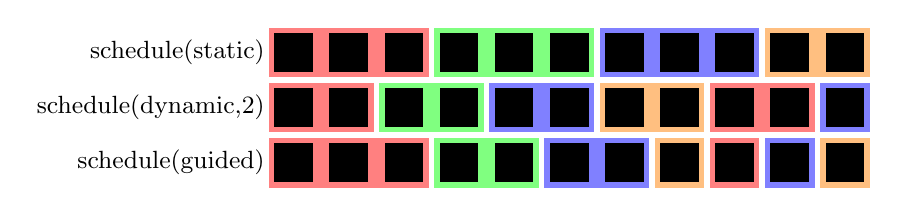
\begin{tikzpicture}[scale=.7]
			\draw (0,.35) node[left]{\small \cdx{schedule(static)}};
			\fill[red!50] (-.1,-.1) rectangle +(2.9,.9);
			\fill[green!50] (2.9,-.1) rectangle +(2.9,.9);
			\fill[blue!50] (5.9,-.1) rectangle +(2.9,.9);
			\fill[orange!50] (8.9,-.1) rectangle +(1.9,.9);
			\draw (0,-.65) node[left]{\small \cdx{schedule(dynamic,2)}};
			\fill[red!50] (-.1,-1.1) rectangle +(1.9,.9);
			\fill[green!50] (1.9,-1.1) rectangle +(1.9,.9);
			\fill[blue!50] (3.9,-1.1) rectangle +(1.9,.9);
			\fill[orange!50] (5.9,-1.1) rectangle +(1.9,.9);
			\fill[red!50] (7.9,-1.1) rectangle +(1.9,.9);
			\fill[blue!50] (9.9,-1.1) rectangle +(.9,.9);
			
			\draw (0,-1.65) node[left]{\small \cdx{schedule(guided)}};
			\fill[red!50] (-.1,-2.1) rectangle +(2.9,.9);
			\fill[green!50] (2.9,-2.1) rectangle +(1.9,.9);
			\fill[blue!50] (4.9,-2.1) rectangle +(1.9,.9);
			\fill[orange!50] (6.9,-2.1) rectangle +(.9,.9);
			\fill[red!50] (7.9,-2.1) rectangle +(.9,.9);
			\fill[green!50] (8.9,-2.1) rectangle +(.9,.9);
			\fill[blue!50] (8.9,-2.1) rectangle +(.9,.9);
			\fill[orange!50] (9.9,-2.1) rectangle +(.9,.9);
			\foreach \i in {0,1,...,10} {
				\fill (\i,0) rectangle +(.7, .7);
				\fill (\i,-1) rectangle +(.7, .7);
				\fill (\i,-2) rectangle +(.7, .7);
			}
		\end{tikzpicture}
	\end{center}
\end{frame}

\begin{frame}[fragile]{Example: number of prime numbers}
	Computing $\pi(n)$, i.e., the number of primes less than or equals to $n$:
	\begin{ccode}
int n = 100000, not_prime = 2;
#pragma omp parallel for reduction(+:not_prime)
for(int i=2; i < n; i++) {
	for (int j=2; j < i; j++) { // large `i` requires more...
		if (i % j == 0) {
			not_prime++;
			break; // ... But iteration may be very short!
		}
	}
}
printf("Pi(%d) = %d\n", n, n - not_prime);
\end{ccode}
Here, scheduling is clearly interesting (but once again, the compiler cannot know that in advance)
\end{frame}

\begin{frame}[fragile]{Example: number of prime numbers}


\begin{textcode}
$ OMP_NUM_THREADS=4 ./pi
                      default     static    dynamic     guided
      n      pi(n)       time       time       time       time
--------------------------------------------------------------
  65536       6542    0.38501    0.34878    0.21439    0.21869
 131072      12251    1.37137    1.46954    0.82317    0.81649
 262144      23000    4.95654    5.70368    3.97412    3.98117
 524288      43390   19.36867   19.65254   13.46914   12.13314
1048576      82025   73.35597   76.84343   44.77434   44.33497
\end{textcode}
As expected, clear advantage of \cdx{dynamic} and \cdx{guided} over \cdx{static}.
\end{frame}

%\begin{frame}[fragile]{FYI: explicit synchronization}
%	\begin{table}
%		\begin{tabular}{lp{8cm}}
%			\toprule
%			Directive & Result \\
%			\midrule
%			\mintinline{c}{barrier} & Explicit wait point for all threads\\
%			\mintinline{c}{master} & Block of instruction only executed by the master thread\\
%			\mintinline{c}{single} & Block of instruction only executed by one of the thread\\
%			\mintinline{c}{critical} & Critical region, only one thread can execute it at the time. May be named.\\
%			\mintinline{c}{atomic} & Limited to a few operations. Sometimes supported by hardware.\\
%			\bottomrule
%		\end{tabular}
%	\end{table}
%\begin{ccode}
%#pragma omp parallel firstprivate(local_sum)
%{
%	#pragma omp for
%	for(i=0;i<n;i++) { // note: barrier even w/o `{`!
%		local_sum += a[i];
%	} // implicit barrier here, probably not usefull
%	#pragma omp atomic
%	sum += local_sum;
%} // implicit barrier
%\end{ccode}
%One can use \mintinline{c}{#pragma omp for nowait} to lift the barrier.
%\end{frame}

\begin{frame}{Results (\cdx{*axpy})}
\begin{figure}
	\centering
	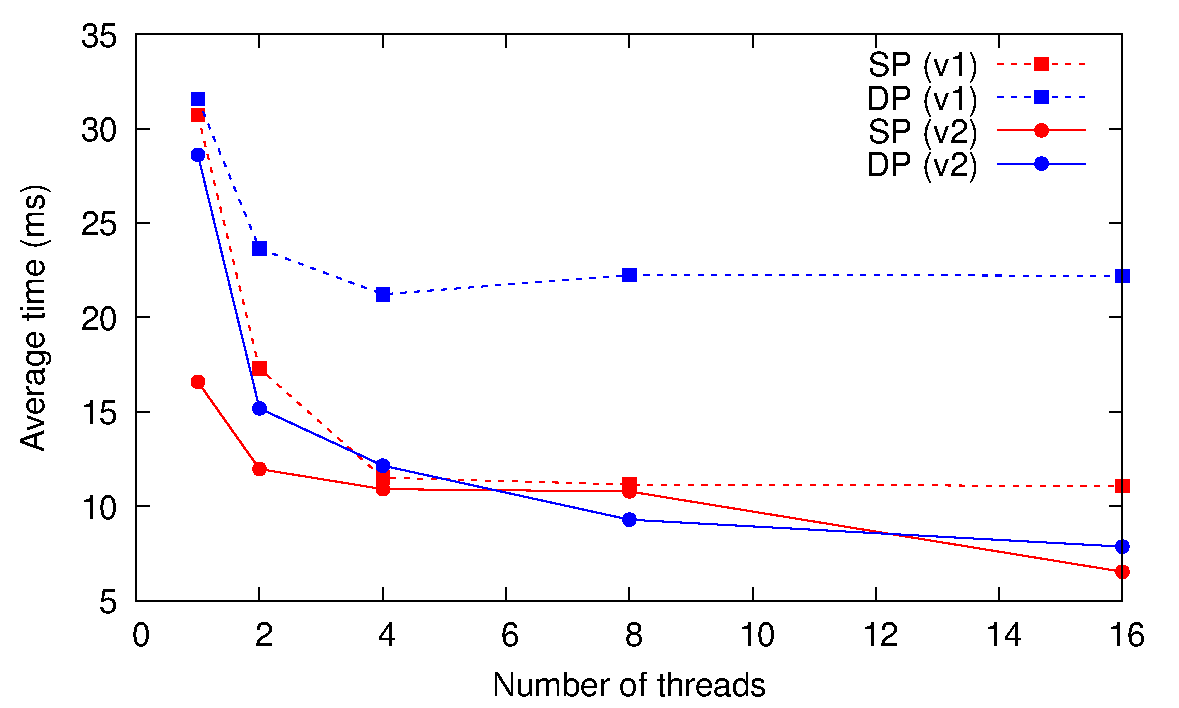
\includegraphics[width=.75\textwidth]{im/result_OMP_saxpy}
	\caption{Results for \cdx{*axpy} ($2^{24}$ numbers) with \cdx{-N 1000} and different values of \cdx{OMP\_NUM\_THREADS}.}
\end{figure}
\begin{itemize}
	\item SP faster than DP.
	\item Modest improvement for 8 and 16 threads (memory bandwidth).
	\item Second version adds SIMD and ``first touch''.
\end{itemize}
\end{frame}

\begin{frame}{Results (\cdx{*dot})}
	\begin{figure}
		\centering
		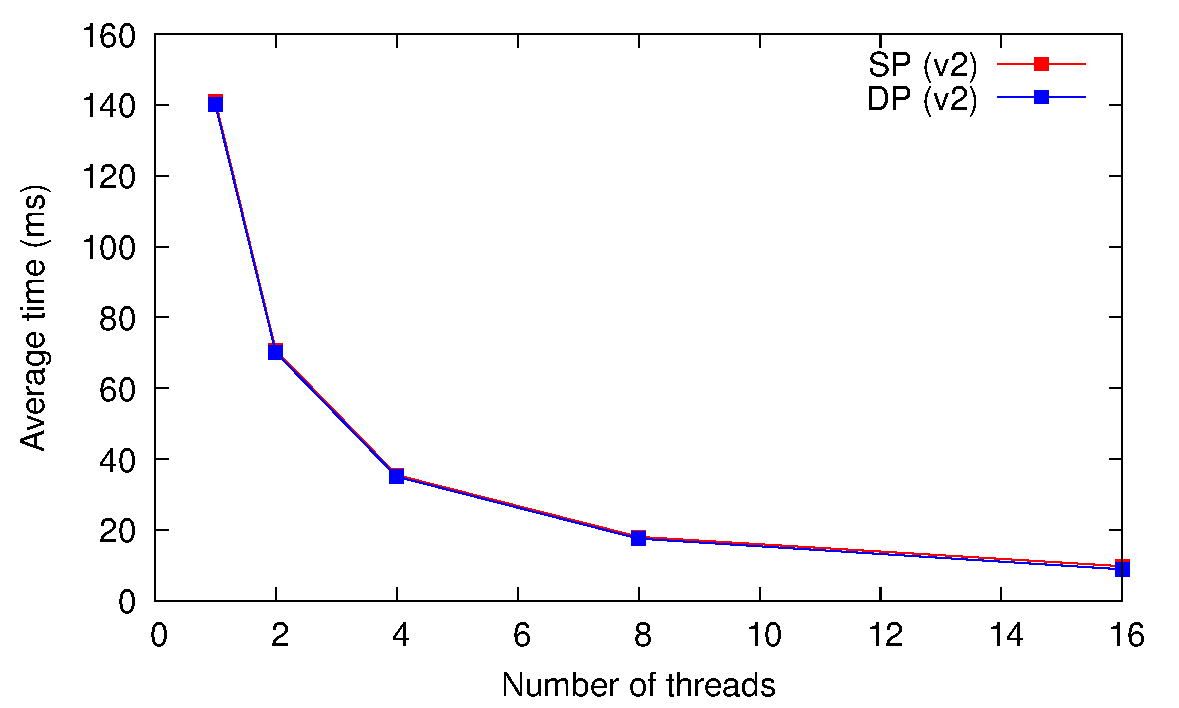
\includegraphics[width=.75\textwidth]{im/result_OMP_dot}
		\caption{Results for \cdx{*dot} ($2^{24}$ numbers) with \cdx{-N 1000} and different values of \cdx{OMP\_NUM\_THREADS}.}
	\end{figure}
\begin{itemize}
	\item Not much difference between SP and DP.
	\item More work intensive loops $\rightarrow$ better speedup with a large number of threads.
\end{itemize}
\end{frame}

\begin{frame}{Going further}
	\begin{itemize}
		\item Explicit synchronization (e.g., \cdx{critical}) ;
		\item Tasks (OpenMP 3.0) for better scheduling: allow parallelizing \cdx{while} loops and recursive call. 
		\item Thread and memory management (NUMA, thread affinity, etc).
	\end{itemize}
\end{frame}
\section{Harder, better, faster, stronger: enrolling other nodes with MPI}

\begin{frame}{MPI?}
	\begin{itemize}
		\item MPI = "message passing interface." It is a communication protocol for programming parallel computers. It defines a common and portable API.
		\item It provides different kinds of communication (point-to-point, collective, one-sided, ...), management, and parallel I/O.
		\item Consequence: sharing the workload is now \textbf{explicit} (and communication is a bottleneck)!
		\item The API is similar to the sockets (\textit{i.e.}, \cdx{open} / \cdx{send} / \cdx{recv} / \cdx{close}), with some improvements:\begin{center}
			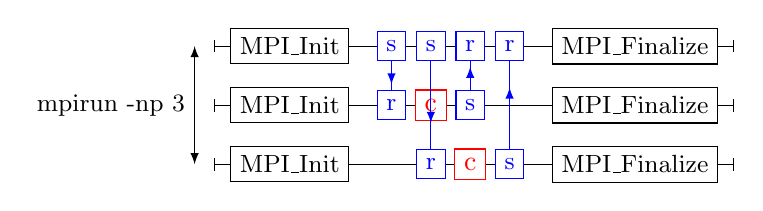
\begin{tikzpicture}
				\draw[latex-latex] (-.25,-.75) -- node[midway,left]{\small \cdx{mpirun -np 3}} + (0,1.5);
				\draw[|-|] (0,.75)  node[right=.2cm,draw,fill=white]{\small \cdx{MPI\_Init}}-- +(6.6,0) node[left=.2cm,draw,fill=white]{\small \cdx{MPI\_Finalize}}; 
				\draw[|-|]  (0,0) node[right=.2cm,draw,fill=white]{\small \cdx{MPI\_Init}}-- +(6.6,0) node[left=.2cm,draw,fill=white]{\small \cdx{MPI\_Finalize}};  
				\draw[|-|]  (0,-.75) node[right=.2cm,draw,fill=white]{\small \cdx{MPI\_Init}}-- +(6.6,0) node[left=.2cm,draw,fill=white]{\small \cdx{MPI\_Finalize}}; 
				\begin{scope}[decoration={
						markings,
						mark=at position 0.65 with {\arrow{latex}}}
					] 
					\draw[postaction={decorate},blue] (2.25,.75) node[draw,fill=white]{\small s} -- +(0,-.75) node[draw,fill=white]{\small r};
					\draw[red] (2.75,0) node[draw,fill=white]{c};
					\draw[postaction={decorate},blue] (2.75,.75) node[draw,fill=white]{\small s} -- +(0,-1.5) node[draw,fill=white]{\small r};
					\draw[postaction={decorate},blue] (3.25,0) node[draw,fill=white]{\small s} -- +(0,.75) node[draw,fill=white]{\small r};
					\draw[red] (3.25,-.75) node[draw,fill=white]{c};
					\draw[postaction={decorate},blue] (3.75,-.75) node[draw,fill=white]{\small s} -- +(0,1.5) node[draw,fill=white]{\small r};
				\end{scope}
			\end{tikzpicture}
		\end{center}
		\item For maximal performances, MPI can be combined with OpenMP.
	\end{itemize}
\end{frame}

\begin{frame}[fragile]{Hello, world!}
\begin{ccode}
#include <mpi.h>
#include <stdio.h>

int main(int argc, char* argv[]) {
	MPI_Init(&argc, &argv);
	int rank, size, len;
	char name[MPI_MAX_PROCESSOR_NAME];
	MPI_Comm_rank(MPI_COMM_WORLD, &rank);
	MPI_Comm_size(MPI_COMM_WORLD, &size);
	MPI_Get_processor_name(name, &len);
	printf("Rank=%d, size=%d (node=%s)\n", rank, size, name);
	MPI_Finalize();
	return 0;
}
\end{ccode}

Processes are grouped into \textbf{communicators}, \textit{i.e.}, a group of processes that can communicate. In such group, each process is assigned a (unique) \textbf{rank}. Default is \cdx{MPI\_COMM\_WORLD} (all processes). The size of the communicator gives the number of processes in this communicator.
\end{frame}

\begin{frame}[fragile]{Compile and run}
	\begin{itemize}
		\item MPI is generally not installed by default and comes in different flavors (implementations). You can install \cdx{openmpi} on your computer.
		\item There is a specific wrapper for the compilation \cdx{mpi[xx]} (which just add the relevant options), \textit{e.g.},\begin{textcode}
mpicc -o hello hello.c
		\end{textcode}
	\item To use the application, you must use the launcher, \cdx{mpirun}, with the number of processes as argument:\begin{textcode}
mpirun -np 2 ./hello
	\end{textcode}
\item With the example given in previous slide, the output is\begin{textcode}
Rank=0, size=2 (node=raspi-cluster-master)
Rank=1, size=2 (node=raspi-cluster-master)
\end{textcode}
	\end{itemize}
\end{frame}

\begin{frame}{Sending}
	MPI passes data in the form of \textbf{messages}. They may be divided in two parts:\begin{enumerate}
		\item Message content: the data to be sent (MPI suppose it is array-like),
		\item The ``envelope'': to which process the message is addressed.
	\end{enumerate}
\begin{center}
	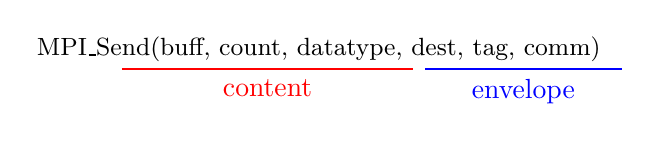
\begin{tikzpicture}
		\draw (0,0) node{\small \cdx{MPI\_Send(buff, count, datatype, dest, tag, comm)}};
		\draw[thick,red] (-2.5,-.25) -- +(3.7,0) node[midway,below]{content};
		\draw[thick,blue] (1.35,-.25) -- +(2.5,0) node[midway,below]{envelope};
	\end{tikzpicture}
\end{center}
The message \cdx{tag} helps to discriminate between different messages addressed to the same process. It is user defined.
\end{frame}

\begin{frame}[fragile]{Sending}
	Sending data to a specific process may be done through one variant of
	\begin{ccode}
MPI_Send(
	void* buff,      // data
	int count,       // number of element to be sent
	MPI_Datatype dt, // type of an element
	int dest,        // recipient (rank)
	int tag,         // type of message
	MPI_Comm c,      // communicator
);
	\end{ccode}
There is also \cdx{MPI\_Isend}, which is \textbf{immediate} (non-blocking). \cdx{dt} may be\begin{itemize}
	\item \cdx{MPI\_CHAR} / \cdx{MPI\_UNSIGNED\_CHAR} (or \cdx{MPI\_BYTE}),
	\item \cdx{MPI\_INT} / \cdx{MPI\_UNSIGNED\_INT},
	\item \cdx{MPI\_LONG} / \cdx{MPI\_UNSIGNED\_LONG},
	\item \cdx{MPI\_FLOAT} / \cdx{MPI\_DOUBLE},
	\item \cdx{MPI\_PACKED} (\textit{i.e.}, \cdx{struct}).
\end{itemize}
\end{frame}

\begin{frame}[fragile]{Receiving}
	Receiving data to a specific process may be done through one variant of
	\begin{ccode}
MPI_Recv(
	void* buff,      // data
	int count,       // number of element to be sent
	MPI_Datatype dt, // type of an element
	int source,      // sender (rank)
	int tag,         // type of message
	MPI_Comm c,      // communicator
	MPI_Status* s    // information on the message
);
	\end{ccode}
	Note that for a communication to succeed, the following should be met:\begin{enumerate}
		\item The same communicator must be used
		\item Source and destination rank must match
		\item The tag must match
		\item The buffer should be large enough on the receive side.
	\end{enumerate}
	Note that \cdx{count} is the \textbf{maximal} number of elements that can be received.
	
\end{frame}

\begin{frame}{Example (ring communication)}
	Ring communication (sent to its next neighbor in the ring, receive from its previous). The goal is, \textit{e.g.}, that every process should have the sum of the ranks at the end:\begin{enumerate}
		\item Set \cdx{sum = 0}, and \cdx{send\_buffer = rank},
		\item Send the buffer to next neighbor, 
		\item Get from the previous in \cdx{receive\_buffer}, adds it to \cdx{sum},
		\item \cdx{send\_buffer = receive\_buffer},
		\item Repeat from step 2 until all ranks have been propagated along the ring.
	\end{enumerate}
\begin{center}
	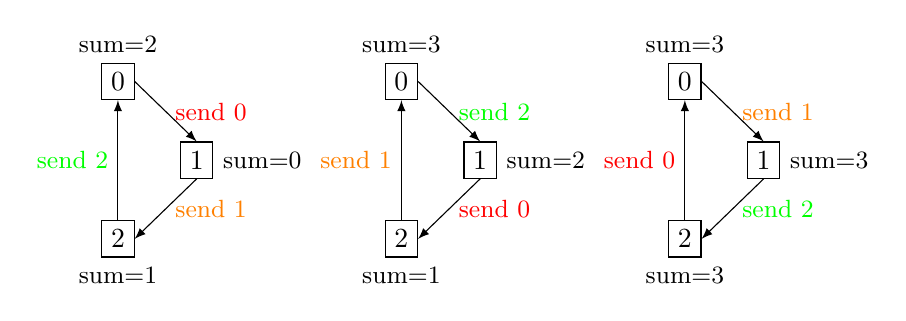
\begin{tikzpicture}[scale=.6]
		\begin{scope}
			\node (x) {};
			\node[above of=x, draw] (x0)  {0};
			\draw (x0.north) node[above] {\small \cdx{sum=2}};
			\node[right of=x,draw] (x1) {1};
			\draw (x1.east) node[right] {\small \cdx{sum=0}};
			\node[below of=x,draw] (x2) {2};
			\draw (x2.south) node[below] {\small \cdx{sum=1}};
			\draw[-latex] (x0.east) -- node[midway,right,red]{\small send 0} (x1.north);
			\draw[-latex] (x1.south) -- (x2.east) node[midway,right,orange]{\small send 1};
			\draw[-latex] (x2.north) -- (x0.south) node[midway,left,green]{\small send 2};
		\end{scope}
	\begin{scope}[xshift=6cm]
	\node (x) {};
	\node[above of=x, draw] (x0)  {0};
	\draw (x0.north) node[above] {\small \cdx{sum=3}};
	\node[right of=x,draw] (x1) {1};
	\draw (x1.east) node[right] {\small \cdx{sum=2}};
	\node[below of=x,draw] (x2) {2};
	\draw (x2.south) node[below] {\small \cdx{sum=1}};
	\draw[-latex] (x0.east) -- node[midway,right,green]{\small send 2} (x1.north);
	\draw[-latex] (x1.south) -- (x2.east) node[midway,right,red]{\small send 0};
	\draw[-latex] (x2.north) -- (x0.south) node[midway,left,orange]{\small send 1};
\end{scope}
\begin{scope}[xshift=12cm]
	\node (x) {};
	\node[above of=x, draw] (x0)  {0};
	\draw (x0.north) node[above] {\small \cdx{sum=3}};
	\node[right of=x,draw] (x1) {1};
	\draw (x1.east) node[right] {\small \cdx{sum=3}};
	\node[below of=x,draw] (x2) {2};
	\draw (x2.south) node[below] {\small \cdx{sum=3}};
	\draw[-latex] (x0.east) -- node[midway,right,orange]{\small send 1} (x1.north);
	\draw[-latex] (x1.south) -- (x2.east) node[midway,right,green]{\small send 2};
	\draw[-latex] (x2.north) -- (x0.south) node[midway,left,red]{\small send 0};
\end{scope}
	\end{tikzpicture}
\end{center}
\end{frame}

\begin{frame}[fragile]{Example (synchronous)}
\begin{ccode}
send_buffer = rank;
for(int i=0; i < comm_size; i++) {
	if (rank % 2 == 0) { // WHY?
		MPI_Send(&send_buffer, 1, MPI_INT, next_rank, rank, 
			MPI_COMM_WORLD);
		MPI_Recv(&receive_buffer, 1, MPI_INT, prev_rank, prev_rank, 
			MPI_COMM_WORLD, MPI_STATUS_IGNORE);
	} else {
		MPI_Recv(&receive_buffer, 1, MPI_INT, prev_rank, prev_rank, 
			MPI_COMM_WORLD, MPI_STATUS_IGNORE);
		MPI_Send(&send_buffer, 1, MPI_INT, next_rank, rank, 
			MPI_COMM_WORLD);
	}
	sum += receive_buffer;
	send_buffer = receive_buffer;
}
\end{ccode}
\end{frame}

\begin{frame}[fragile]{Example (asynchronous)}
Both asynchronous call:
\begin{ccode}
MPI_Request requests[2];
MPI_Isend(&send_buffer, 1, MPI_INT, next_rank, rank, 
	MPI_COMM_WORLD, &requests[0]);
MPI_Irecv(&receive_buffer, 1, MPI_INT, prev_rank, prev_rank, 
	MPI_COMM_WORLD, &requests[1]);
MPI_Waitall(2, requests, MPI_STATUS_IGNORE); // barrier
\end{ccode}
or asynchronous sent followed by synchronous receive:
\begin{ccode}
MPI_Request request;
MPI_Isend(&send_buffer, 1, MPI_INT, next_rank, rank, 
	MPI_COMM_WORLD, &request);
MPI_Recv(&receive_buffer, 1, MPI_INT, prev_rank, prev_rank, 
	MPI_COMM_WORLD, MPI_STATUS_IGNORE);
MPI_Wait(&request, MPI_STATUS_IGNORE); // not required
\end{ccode}

\end{frame}

\begin{frame}[fragile]{Example: ping-pong}
\begin{ccode}
long N = 2 << i;
double* A = calloc(N, sizeof(double));
elapsed = MPI_Wtime();
for(int k=0; k < N_PING_PONG; k++) {
	if (rank == 0) {
		MPI_Send(A, N, MPI_DOUBLE, 1, 0, 
			MPI_COMM_WORLD);
		MPI_Recv(A, N, MPI_DOUBLE, 1, 0, 
			MPI_COMM_WORLD, MPI_STATUS_IGNORE);
	} else {
		MPI_Recv(A, N, MPI_DOUBLE, 0, 0, 
			MPI_COMM_WORLD, MPI_STATUS_IGNORE);
		MPI_Send(A, N, MPI_DOUBLE, 0, 0, 
			MPI_COMM_WORLD);
	}
}
elapsed = MPI_Wtime() - elapsed;
\end{ccode}
Elapsed time depends on the amount of data and asymptotically tend to the bandwith.
\end{frame}

\begin{frame}{Example: ping-pong}
	\begin{figure}
		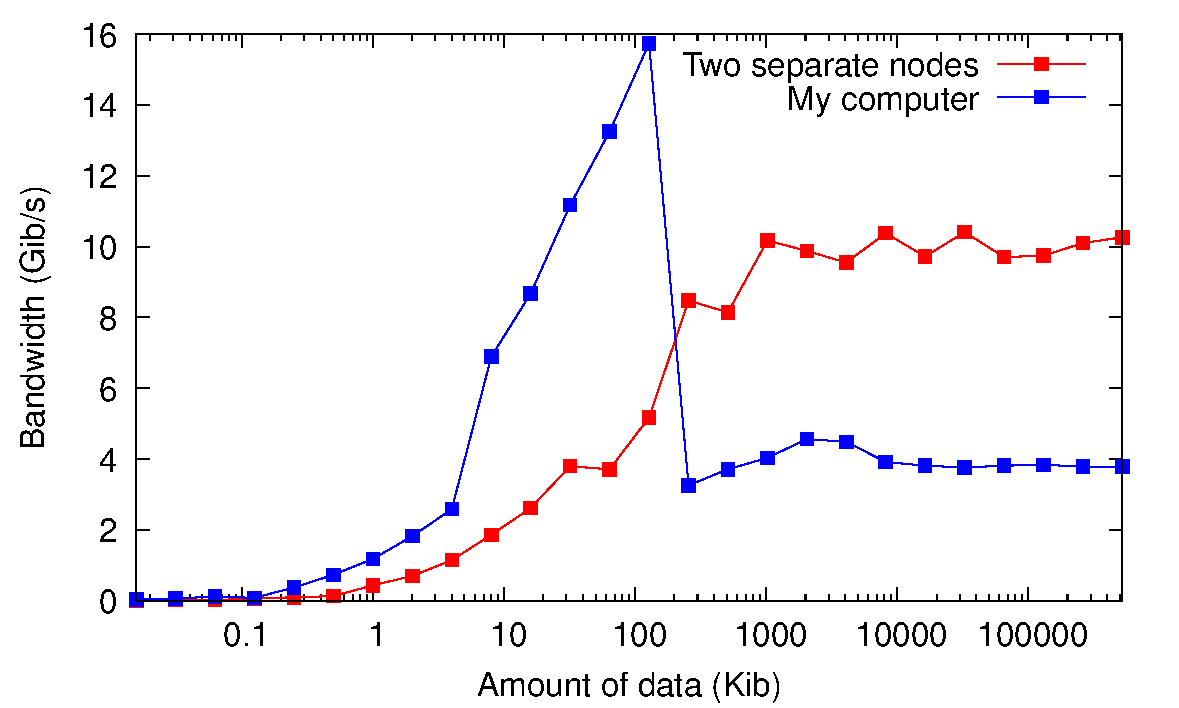
\includegraphics[width=.85\textwidth]{im/result_MPI_ping}
		\caption{Bandwidth, as measured by the ping-pong example, in two different configurations}
	\end{figure}
What (the hell!) did happen in both cases?
\end{frame}

\begin{frame}{Other ways to communicate}
	\begin{center}
		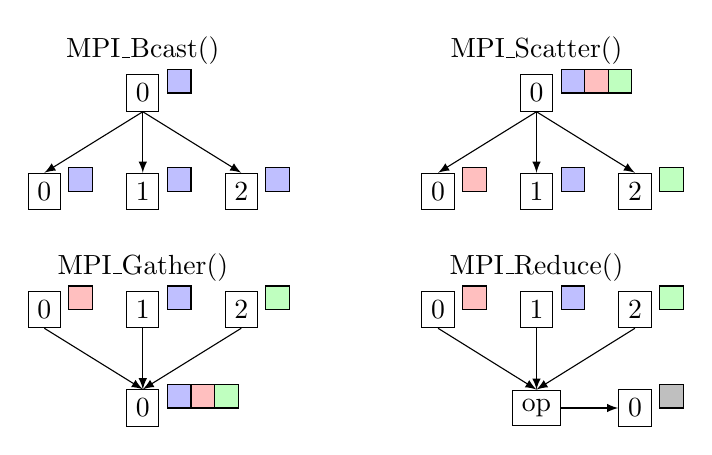
\begin{tikzpicture}[node distance=1.25cm]
			\begin{scope}
				\node[draw] (x0) {0};
				\draw (x0.north) node[above]{\cdx{MPI\_Bcast()}};
				\draw[fill=blue!25] (x0.east) ++(.1,0) rectangle ++(.3,.3);
				\node[below of=x0,draw] (y1) {1};
				\draw[fill=blue!25] (y1.east) ++(.1,0) rectangle ++(.3,.3);
				\node[left of=y1,draw] (y0) {0};
				\draw[fill=blue!25] (y0.east) ++(.1,0) rectangle ++(.3,.3);
				\node[right of=y1,draw] (y2) {2};
				\draw[fill=blue!25] (y2.east) ++(.1,0) rectangle ++(.3,.3);
				\draw[-latex] (x0.south) --(y0.north);
				\draw[-latex] (x0.south) --(y1.north);
				\draw[-latex] (x0.south) --(y2.north);
			\end{scope}
		\begin{scope}[xshift=5cm]
		\node[draw] (x0) {0};
		\draw (x0.north) node[above]{\cdx{MPI\_Scatter()}};
		\draw[fill=blue!25] (x0.east) ++(.1,0) rectangle ++(.3,.3);
		\draw[fill=red!25] (x0.east) ++(.4,0) rectangle ++(.3,.3);
		\draw[fill=green!25] (x0.east) ++(.7,0) rectangle ++(.3,.3);
		\node[below of=x0,draw] (y1) {1};
		\draw[fill=blue!25] (y1.east) ++(.1,0) rectangle ++(.3,.3);
		\node[left of=y1,draw] (y0) {0};
		\draw[fill=red!25] (y0.east) ++(.1,0) rectangle ++(.3,.3);
		\node[right of=y1,draw] (y2) {2};
		\draw[fill=green!25] (y2.east) ++(.1,0) rectangle ++(.3,.3);
		\draw[-latex] (x0.south) --(y0.north);
		\draw[-latex] (x0.south) --(y1.north);
		\draw[-latex] (x0.south) --(y2.north);
	\end{scope}
\begin{scope}[yshift=-4cm]
\node[draw] (x0) {0};
\draw[fill=blue!25] (x0.east) ++(.1,0) rectangle ++(.3,.3);
\draw[fill=red!25] (x0.east) ++(.4,0) rectangle ++(.3,.3);
\draw[fill=green!25] (x0.east) ++(.7,0) rectangle ++(.3,.3);
\node[above of=x0,draw] (y1) {1};
\draw (y1.north) node[above]{\cdx{MPI\_Gather()}};
\draw[fill=blue!25] (y1.east) ++(.1,0) rectangle ++(.3,.3);
\node[left of=y1,draw] (y0) {0};
\draw[fill=red!25] (y0.east) ++(.1,0) rectangle ++(.3,.3);
\node[right of=y1,draw] (y2) {2};
\draw[fill=green!25] (y2.east) ++(.1,0) rectangle ++(.3,.3);
\draw[-latex] (y0.south) --(x0.north);
\draw[-latex] (y1.south) --(x0.north);
\draw[-latex] (y2.south) --(x0.north);
\end{scope}
\begin{scope}[yshift=-4cm,xshift=5cm]
	\node[draw] (x0) {op};
	\node[right of=x0,draw] (x1) {0};
	\draw[fill=black!25] (x1.east) ++(.1,0) rectangle ++(.3,.3);
	\node[above of=x0,draw] (y1) {1};
	\draw (y1.north) node[above]{\cdx{MPI\_Reduce()}};
	\draw[fill=blue!25] (y1.east) ++(.1,0) rectangle ++(.3,.3);
	\node[left of=y1,draw] (y0) {0};
	\draw[fill=red!25] (y0.east) ++(.1,0) rectangle ++(.3,.3);
	\node[right of=y1,draw] (y2) {2};
	\draw[fill=green!25] (y2.east) ++(.1,0) rectangle ++(.3,.3);
	\draw[-latex] (y0.south) --(x0.north);
	\draw[-latex] (y1.south) --(x0.north);
	\draw[-latex] (y2.south) --(x0.north);
	\draw[-latex] (x0.east) --(x1.west);
\end{scope}
		\end{tikzpicture}
	\end{center}
... And others (asynchronous \cdx{I*}, All-to-all \cdx{All*}, vectors \cdx{*v}, ...).
\end{frame}

\begin{frame}{Results}
	\begin{figure}
		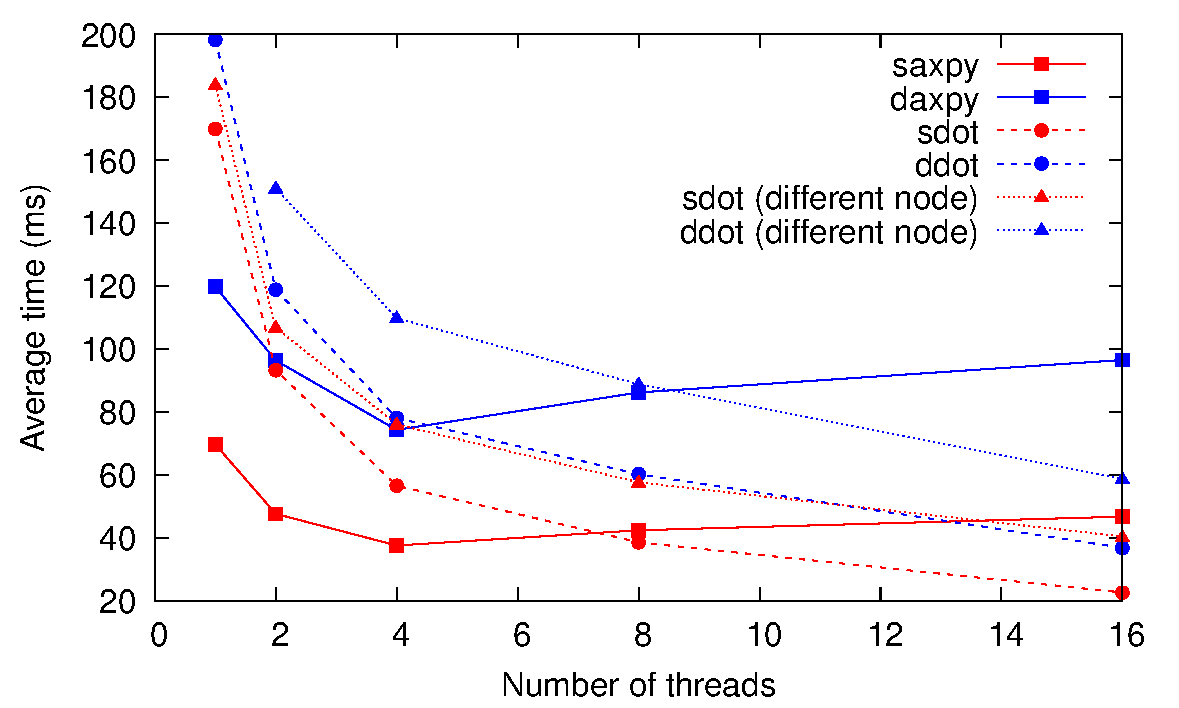
\includegraphics[width=.75\textwidth]{im/result_MPI}
		\caption{Results ($2^{24}$ numbers) with \cdx{-N 1000} and different number of processes.}
	\end{figure}
\begin{itemize}
	\item Not so good in general.
	\item Again, more interesting for \cdx{*dot} (more work intensive) than for \cdx{*axpy} (bandwidth limited).
	\item Thanks to Infiniband, not so much impact when different nodes are used.
\end{itemize}
\end{frame}
\section{Next gen' stuffs: the GPUs}

\begin{frame}{Why? How?}
	\begin{itemize}
		\item CPU and GPU actually took different paths:\begin{itemize}
			\item A CPU is very general purpose, with a complex set of operation (and prediction / speculative execution) and high clock rate.
			\item A GPU is designed for \textit{data stream}, by having a whole bunch of ALU, designed for bulk data handling. Thanks to Joule's law, the clock rate has to be smaller.
		\end{itemize}
		\item There are different approaches to program with GPUs:\begin{enumerate}
			\item Specific: NVIDIA CUDA, AMD HIP,
			\item Explicit cross-platform: OpenCL,
			\item Directive based: OpenACC, \textbf{OpenMP}.
		\end{enumerate}
	\item Though it is generally less difficult to manage (there is generally one device), communication is still the issue.
	\item Of course, I will use OpenMP (which actually uses CUDA/HIP as back-end). It works with \cdx{gcc}, but you will probably get better performances with \cdx{clang}.
	\end{itemize}
\end{frame}

\begin{frame}{A bit of (confusing) terminology}
	\begin{table}
		\begin{tabular}{lll}
			\toprule
			OpenMP & NVIDIA & AMD\\
			\midrule
			SIMD Lane & Thread & Work item \\
			Thread & Warp &  Wavefront \\
			Team & Thread block & Workgroup\\ 
			League & Grid & ?? \\
			\bottomrule
		\end{tabular}
	\end{table}
	\begin{itemize}
		\item Each ``worker'' control SIMD lanes of size $L_v$, (each one of them being generally referred to as a \textit{thread}, executed by a \textit{core})
		\item the $N_w$ workers are grouped into a \textbf{team},\footnote{This is the OpenMP terminology} (thus containing $L_v \times N_w$ cores). On CPU, there was only one team.
		\item There are up to $N_t$ teams that work independently. This is where new instructions are needed.
	\end{itemize}
\end{frame}

\begin{frame}[fragile]{Offload and distribute}
	\begin{itemize}
		\item To offload code to GPU, use \cdx{omp target}.
		\item To create a collection (league) of teams, use \cdx{omp teams}. As usual, parallel $\neq$ worksharing.
		\item To distribute iterations over the teams, use \cdx{omp distribute}.
		\item Combine that with the usual instruction to further distribute over threads.
	\end{itemize}
\begin{ccode}
#pragma omp target
{
	// distributed over all thread of all teams:
	#pragma omp teams distribute parallel for
	for(int i=0; i < N; i++) 
		x[i] = 2.0 * x[i];
}
\end{ccode}
Actually, this code may not work...
\end{frame}

\begin{frame}[fragile]{Data management}
	OpenMP  (in some implementation\footnote{At least GCC 10}) needs to know which data to move to and from the GPU. Use the \cdx{map} clause:\begin{itemize}
		\item \cdx{map(to: list)}: copy data to GPU,
		\item \cdx{map(from: list)}: copy data from GPU,
		\item \cdx{map(tofrom: list)}: copy data to and from the GPU,
		\item  \cdx{map(alloc: list)}: directly allocate data on the GPU.
	\end{itemize}
\begin{ccode}
#pragma omp target map(tofrom: x[0:N])
{
	#pragma omp teams distribute parallel for
	for(int i=0; i < N; i++)
		x[i] = AX * x[i];
}
\end{ccode}
Notice that for an array, we have to give the number of data (since it may be a dynamic allocation). Use \cdx{target data} for permanent data management.
\end{frame}

\begin{frame}{Results}
\begin{table}
	\begin{tabular}{l cc c cc}
		\toprule
		& \multicolumn{2}{c}{\cdx{*dot}} &&\multicolumn{2}{c}{\cdx{*axpy}}\\
		& \cdx{s} & \cdx{d} && \cdx{s} & \cdx{d}\\
		\midrule
		Serial (\cdx{-O1}) & 141.1 & 140.1  && 30.7 & 31.7\\
		OMP CPU (4) & 35.5 & 35.0 & & 10.9 & 12.1 \\
		OMP GPU & 47.0& 54.8 && 52.3& 75.6 \\
		\bottomrule
	\end{tabular}
	\caption{Average running times (in ms) with \cdx{-N 1000}, on $2^{24}$ numbers.}
\end{table}
\begin{itemize}
	\item Compiled with \cdx{gcc -o xxx xxx.c -O1 -lm -fopenmp -foffload=-misa=sm\_35}, with CUDA 11.1.
	\item Ran on NVIDIA RTX 2080 (should be \cdx{sm\_75}!).
	\item And, well, that's awful... Again ``thanks'' to data transfer.
\end{itemize}
\end{frame}

\begin{frame}{But wait, there is more! Introducing... Laplace.}
	\begin{columns}
	\column{.6\textwidth}
	\begin{itemize}
		\item Laplace's equation: $\nabla^2 U = 0$. Used to model the diffusion phenomenons: $U$ is unknown.
		\item A very common approximation is the iterative procedure based on the (Jacobi) 4-point stencil. One a grid with evenly spaced (of $h$) points, it reduces to\begin{align*}
			&U^{k+1}(x,y) = \\
			&\hspace{.5cm}\frac{U^k(x\pm h,y)+U^k(x,y\pm h)}{4}.
		\end{align*}
		where $k$ is the iteration number.
		\item The values at the borders are fixed (Dirichlet)
		\item Excellent for GPU (or MPI): after upload, the data remains and are updated.
		\end{itemize}
	\column{.4\textwidth}
	\begin{figure}
		\centering
		
\includegraphics[width=\textwidth]{im/Laplace}
		\caption{Visualization of $U$ after 10 000 iterations on a 512x512 grid ($h=1$).}
	\end{figure}
	\end{columns}
\end{frame}

\begin{frame}{Results}
	\begin{figure}
		\centering
		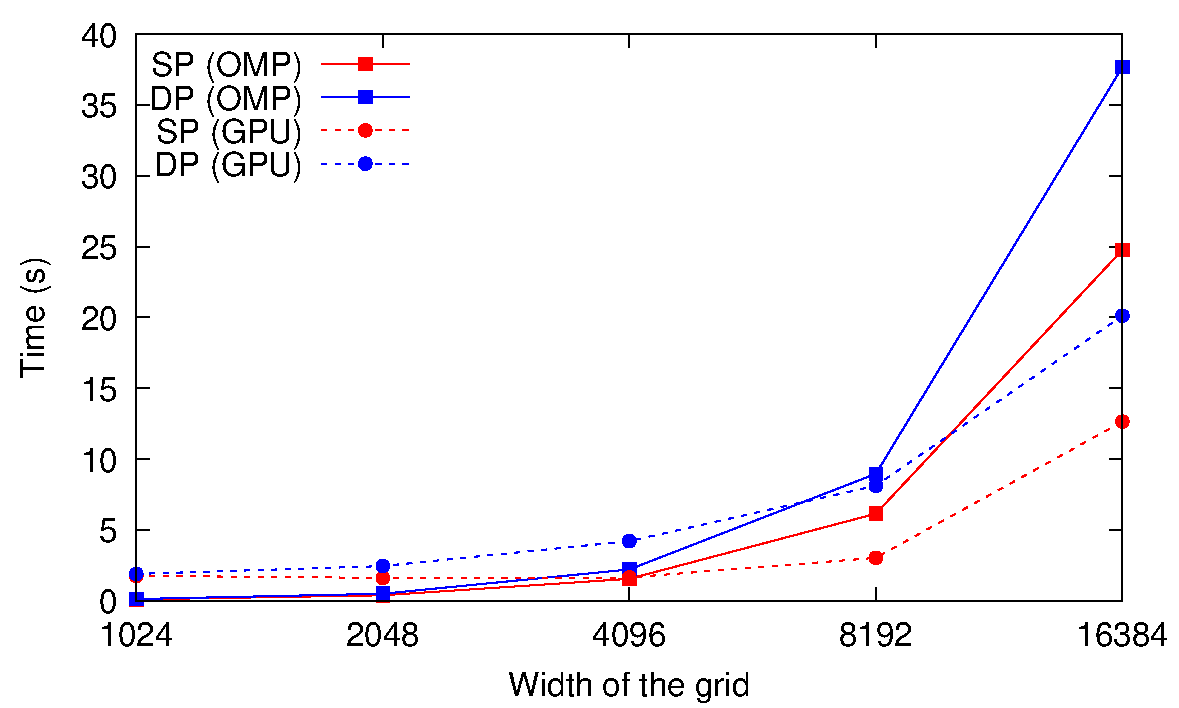
\includegraphics[width=.85\textwidth]{im/result_GPU_Laplace}
		\caption{Results for the first 200 iteration with the size of the grid of the Laplace procedure on a CPU (with \cdx{OMP\_NUM\_THREADS=4}) and a GPU.}
	\end{figure}
	Now that gets interesting! 
\end{frame}
\section{The end of the beginning}

\begin{frame}{To conclude}
	\begin{itemize}
		\item Again, optimization is an art! My goal was actually twofold:\begin{enumerate}
			\item Convince you that compiler knows better than you, and
			\item Convince you that the directive approach allows you to gradually improve performance without (much) of rewrite.
		\end{enumerate}
		\item There is a clear trend towards GPUs, so the support will improve in the future (and a standard will probably emerge\footnote{It may already be there, with all libraries copying the CUDA style.}). You just need to avoid data transfer as much as possible.
		\item This was just an introduction, so take a look around! The CÉCI is organizing training if you are interested to go further (\url{http://www.ceci-hpc.be/training.html}), and there is a student cluster at UNamur (called Hyades) if you want to play (in the frame of a lecture, though).
		\item If you really want to explore the topic, keep in mind that other languages also have concurrent tasks directly available as part of the language...
		\end{itemize}
\end{frame}

\end{document}
